\chapter{GEREKSİNİM ANALİZİ} \label{chapter:gereksinimAnalizi}
OpenCL ve CUDA altyapıları kullanılarak gerçeklenen sinyal işleme uygulamalarının, özelleştirilebilir, milli tasarım bir donanım üzerinde çalıştırılması amacı ile başlatılan projenin gerekinimleri \ref{projeGereksinimleri} Proje Gereksinimleri başlığı altında sunulmuştur. \ref{paralellestirmeninBasarimaEtkisi} Paralelleştirmenin Başarıma Etkisi başlığı altında proje için performans metrikleri belirlenmiş, \ref{fonksiyonlarinGerceklenmesi} Fonksiyonların Gerçeklenmesi başlığı altında, Tablo \ref{table:fonksiyonListesi}: Fonksiyon Listesi tablosunda verilen fonksiyonların matematiksel ifadeleri ve sayısal sistemler üzerinde gerçekleme algoritmaları sunulmuştur. Sunulan ifadeler \ref{chapter:mimariTasarimi} bölümünde kullanılacaktır. 
\newpage
\section{Proje Gereksinimleri} \label{projeGereksinimleri}
 Proje gereksinimleri şu şekildedir: 
\begin{enumerate}
  \item Tasarlanan işlemci çok çekirdekli mimariye sahip olmalıdır.
  \item Tasarlanan işlemcinin buyruk kümesi OpenCL 1.2 desteklemelidir. 
  \item Tüm işlemler 32 bit integer ve floating point sayılar üzerinden yapılmalıdır. Floating point sayılar için IEEE754 standardı kullanılmalıdır.
  \item Tasarım modüler olmalı alt modül sayıları parametrik tanımlanmalı, bütün mimari modülleri özelleştirilebilir olmalıdır. 
  \item Gelecek çalışmalarda tasarlanacak özel hesaplama ipcore modülleri için standart bir arayüzü desteklemelidir.
  \item Tasarım sayısal sinyal işleme uygulamalarında sıklıkla kullanılan ve Tablo \ref{table:fonksiyonListesi} içinde belirtilen fonksiyonları desteklemelidir.
  \item Verilen bir matrisin kopyası oluşturulup kopya üzerinden işlem yapılmalıdır.
  \item Reel sayılar matrisi oluşturulurken bellekte yalnızca reel sayıların sığabileceği bir alan kullanılmalıdır, karmaşık sayılar matrisi oluşturulurken reel ve imajiner kısımlar için ayrı yer ayrılmalıdır.
  \item Satır, sütun veya alt matris üzerinde işlem yapılırken yalnızca ilgili veriler kopyalanmalıdır.
  \newpage
  	
  
\end{enumerate}

\begin{longtable}{p{80pt} p{250pt}}
\caption[Desteklenmesi beklenen fonksiyon listesi]{Desteklenmesi beklenen fonksiyon listesi} \label{table:fonksiyonListesi} \\
\multicolumn{1}{c}{\textbf{Fonksiyon}} & \multicolumn{1}{c}{\textbf{Açıklama}} \\ 
\hline 
\endfirsthead

\multicolumn{2}{c}%
{{\bfseries \tablename\ \thetable{} -- devam}} \\
\multicolumn{1}{c}{\textbf{Fonksiyon}} &
\multicolumn{1}{c}{\textbf{Açıklama}}  \\ \hline 
\endhead

\hline \multicolumn{2}{r}{{Sonraki sayfada devam etmektedir.}} \\ 
\endfoot

\hline \hline
\endlastfoot
 Toplama 								& İki matrisin eleman eleman toplanması 											\\%math_desc%		& C$_{m,n}$=A$_{m,n}$ + B$_{m,n}$  \\
 												& Matrisin tüm elemanlarına sabit eklenmesi										\\%math_desc% 		& C$_{m,n}$= A$_{m,n}$ + b  \\
 Çıkarma 								& İki matrisin eleman eleman farkı 														\\%math_desc		& C$_{m,n}$= A$_{m,n}$ - B$_{m,n}$ \\
 												& Matrisin tüm elemanlarından sabit çıkarılması 							\\%math_desc		& C$_{m,n}$= A$_{m,n}$ - b\\
 Çarpma									& Matrislerin eleman - eleman çarpımı 												\\%math_desc		& C$_{m,n}$= A$_{m,n}$ * B$_{m,n}$\\
 												& Matris çarpımı 																							\\%math_desc		& C = A x B\\
 												& Matrisin tüm elemanlarının sabit ile çarpımı				 				\\%math_desc		& C$_{m,n}$= A$_{m,n}$ * b\\
 Bölme									& Matrislerin eleman - eleman bölümü 													\\%math_desc		& C$_{m,n}$= A$_{m,n}$ / B$_{m,n}$\\
 												& Matrisin tüm elemanlarının sabite bölümü 						 				\\%math_desc		& C$_{m,n}$= A$_{m,n}$ / b\\
 Toplam									& Matrisin satır toplamları 																	\\%math_desc		& C$_{(mx1)}$=sum(A,rows)\\
 												& Matrisin sütun toplamları				 														\\%math_desc		& C$_{(1xn)}$=sum(A,cols)\\
 												& Matrisin tüm elemanlarının toplamı 													\\%math_desc		& C = sum(A)\\
 Max, Min,  						& Her satır için																							\\%math_desc		& \\
 Mean, Median						& Her sütun için																							\\%math_desc		& \\
 												& Matrisin tüm elemanları için																\\%math_desc		& \\
 												& En büyük elemanın ilk indisi																\\%math_desc		& \\
 												& Mutlak en büyük elemanın değeri															\\%math_desc		& \\
 												& Mutlak en büyük elemanın ilk indisi													\\%math_desc	  & \\
 Nokta çarpımı					& İki vektörün nokta çarpımı																	\\%math_desc		& C = V$_{1}$ . V$_{2}$\\
 FFT/IFFT								& Her satırın fourier ve ters fourier dönüşümü								\\%math_desc		& \\
 												& Her sütunun fourier ve ters fourier dönüşümü								\\%math_desc		& \\
 Logaritma							& Her eleman için doğal logaritma hesabı											\\%math_desc		& C$_{m,n}$ = ln(A$_{m,n}$)\\	
 												& Her elemean için 10 tabanında logaritma hesabı							\\%math_desc		& C$_{m,n}$ = log10(A$_{m,n}$)\\
 Eksponansiyel					& 10 tabanında eksponansiyel 																	\\%math_desc		& C$_{m,n}$ = 10$^{A_{m,n}}$\\
 												& Doğal tabanda eksponansiyel 																\\%math_desc		& C$_{m,n}$ = e$^{A_{m,n}}$\\ 
 Büyüklüğü  						& Matrisin mutlak büyüklüğü																		\\%math_desc		& C = mag(A, abs)\\ 
 												& Matrisin enerjisi																						\\%math_desc		& C = mag(A, sqr) \\	
 Evrişim 								& Dairesel konvolüsyon (Circular convolution)									\\%math_desc		& C = cconv(A, B, n)\\ 
 												& Doğrusal konvolüsyon (Linear convolution) 									\\%math_desc		& C = conv(A, B, n)\\  
 Eşlenik     						&	Bir matrisin karmaşık eşleniği															\\%math_desc		& C = conj(A)\\
 Transpoz								&	Bir matrisin transpozu																			\\%math_desc		& B = A'\\
 											  &	Bir matrisin eşleniksiz transpozu														\\%math_desc		& B = A.'\\			
 Determinant						& Bir kare matrisin determinantı															\\%math_desc		& C = det(A)\\
 Trigonometrik					& Her eleman için sin/cos/tan değerleri 											\\%math_desc		& \\ 			
 Filtreleme							& Her satırı FIR ve IIR Filtreleme 														\\%math_desc		& \\
 												& Her sütunu FIR ve IIR Filtreleme 														\\%math_desc		& \\
 Windowing 							& Hamming, Hanning ve Gaussian 																\\%math_desc		& \\
 Alt matris 						& Matrisin bir satırını al / değiştir   											\\%math_desc		& \\
 												& Matrisin bir sütununu al / değiştir													\\%math_desc		& \\
 												& Matrisin bir alt matrisini al / değiştir										\\%math_desc		& \\
 Türev									& Bir vektörün 1. derecede türevi															\\%math_desc		& \\
 Norm 									& Matrisin ve vektörün p. dereceden normu 										\\%math_desc		& \\
 Sıralama 							& Satır sıralama 																							\\%math_desc		& \\
 												& Sütun sıralama 																							\\%math_desc		& \\
 												& Matris sıralama (vektör sıralama gibi) 											\\%math_desc		& \\
 Varyans,								& Satır bazlı 	 																							\\%math_desc		& \\
 Standart Sapma					& Sütun bazlı 	 																							\\%math_desc		& \\
 												& Matris bazlı 	 																							\\%math_desc		& \\
 İşaret									& Her bir eleman için signum fonksiyonu 											\\%math_desc		& \\
 Flip										& Yatay ve düşey eksende flip 																\\%math_desc		& \\
 Karekök 								& Her eleman için karekök 																		\\%math_desc		& \\
 Reverse 								& Elemanların sırasını tersine çevirir 												\\%math_desc		& \\
 Interpolasyon 					& Lineer interpolasyon 																				\\%math_desc		& \\
 Karşılaştırma 					& Satır, sütun bazlı veya matris için karşılaştırma 					\\%math_desc		& 
\end{longtable}

Tasarlanan donanımın temel tasarım kararlarını oluşturan gereksinimler ve fonksiyon listesi incelenmiş, her bir matematiksel işlem için gerekli buyruklar ve donanım birimleri belirlenmiştir. 


\section{Paralelleştirmenin Başarıma Etkisi}
Tablo \ref{table:fonksiyonListesi} içinde belirtilen işlemlerin paralelleştirilmesi ile işlem sürelerinin kısalması beklenmektedir. Paralel hesaplamada işlem süresini belirleyen 4 unsur vardır. \par

Bunlardan birincisi bellek işlemlerine ayrılan süredir. Programlanabilir her sistemde olduğu gibi bir işlem veya işlem dizisi başlarken bellekten veri okunur, sonlandığında ise tekrar belleğe sonuçlar yazılır. İşlemler paralelleştirilse de paralelleştirilmese de bellek için harcanan süre toplamda yakındır. {Citation Here} Hem yazılım hem de donanım seviyesinde bellek işlemlerinde yerelliği artırmak bellek işlemlerinin daha hızlı işlenmesine olanak sağlar.\par

İkinci unsur paralelleştirmenin bir ölçüsü olan thread sayısıdır. Söz konusu işlem birbirinden bağımsız iş parçacıklarına bölünür ve her bir iş parçacığı farklı donanımlarda koşturularak paralel işleme sağlanır. Literatürde bu iş parçacıkları ingilizce ismi olan thread kelimesiyle ifade edilmekte ve thread kelimesinin buradaki anlamını taşıyan bir türkçe tercümesi bulunmamaktadır. Bu sebeple tezin devamında sürekli olarak thread kelimesi kullanılacaktır. Thread sayısındaki artış, programın daha paralel koşturulabilmesine olanak sağlar.\par

Üçüncü unsur donanımda gerçeklenmiş thread yolu sayısıdır. Her bir thread, bir thread yoluna atanır ve o yol üzerinde koşturulur. Eğer thread yolu sayısı thread sayısından büyük veya eşitse, tek seferde bütün threadler işlenir ve program sonlanır. Eğer thread sayısı, thread yolu sayısından fazla ise threadler, thread yolu sayısı kadar elemana sahip kümelere bölünür. NVidia'nın dokümanlarında warp ismi ile anılan bu thread kümelerinin her biri tek seferde işlenir. Toplam işlem süresi ise warp sayısına bağlı olarak artar. Thread yolu sayısının artırılması warp sayısında ve işlem süresinde azalmaya yol açar. Ancak fiziksel kısıtlardan dolayı thread yolu sayısının bir üst limiti vardır. \par

Dördüncü unsur ise her bir thread için harcanan yürütme zamanıdır. Thread başına düşen yürütme zamanı thread içindeki buyruk sayısına, buyrukların çevrim sayılarına, buyruklar arası veri bağımlılıklarına, işlemcinin boru hattı mimarisine ve işlemcinin frekansına bağlı olarak değişir.\par

Dolayısıyla bir paralelleştirilmiş bir uygulamanın yürütme zamanı denklem \ref{equation:yurutmeZamani}'de gösterildiği şekilde formüle dökülebilir.

\begin{equation} \label{equation:yurutmeZamani}
t_{program} = t_{bellek} + t_{thread} x \frac{N_{thread}}{N_{thread yolu}} \& 
t_{thread} = N_{buyruk} x c_{ortalama} x T_{saat}
\end{equation} 

Burada $t_{program}$ program süresini, $t_{bellek}$ bellek işlemleri süresini, $t_{thread}$ thread süresini, $N_{thread}$ toplam thread sayısını, $N_{thread yolu}$ toplam thread yolu sayısını, $N_{buyruk}$ thread içindeki buyruk sayısını, $c_{ortalama}$ her buyruk için harcanan çevrim sayılarının ortalamasını, $T_{saat}$ işlemci saatinin periyodunu ifade eder.\par

Thread yolu sayısının 1 olduğu durumda aynı anda tek bir thread işlenebilir. Dolayısıyla işlem paralelleştirilmemiş olur. Thread yolu sayısının sonsuza gitmesi halinde ise program süresi bellek işlemleri için harcanan zamana eşit olur. \par
\textbf{Program süresi bileşenlerinin optimize edilmesi}\par
Thread sayısı ve thread içindeki buyruk sayısı yazılım katmanında belirlenen değerlerdir. Bellek işlemleri için harcanan süre kaçınılmaz olmasına rağmen yazmaç öbeği, paylaşımlı bellek ve ana bellek ara yüzü gibi load ve store işlemleri ile ilgili donanımların tasarımlarında yapılan iyileştirmeler bellek için harcanan süreyi azaltabilir. Öte yandan işlemci frekansı ve işlemler için harcanan ortalama çevrim sayıları da hesaplama işlemlerinin süresini doğrudan belirleyen bileşenler olup optimize edilmesi gerekmektedir. Bu tarz bir optimizasyon için buyruk kümesi ve boru hattı mimarisi belirleyici yapılardır. Buyruk kümesi tasarımı için fonksiyon listesinde bulunan işlemler \par 

\section{Fonksiyonların Gerçeklenmesi} \label{fonksiyonlarinGerceklenmesi}
Fonksiyon listesinde belirtilen fonksiyonların tamamında veriler bellekten okunmakta ve sonuçlar yine belleğe yazılmaktadır. Dolayısıyla load ve store işlemleri fonksiyonlrın tümünde olmalıdır. Her bir fonksiyon için gerekli buyruklar ise her fonksiyonun kendi başlığı altında belirtilmiştir.

\subsection{Toplama işlemi}
İki matrisin eleman eleman toplamında her bir thread $C_{i,j} = A_{i,j} + B_{i,j}$ işlemini yapar. Bu işlem için ihtiyaç duyulan buyruklar floating point ve integer toplama buyruklarıdır. Bir matrisin sabit sayı ile toplanması durumunda ise her bir thread $C_{i,j} = A_{i,j} + k$ işlemini yapar. Burada k değeri integer veya floating point bir sayı olup, bellekten okunabileceği gibi anlık olarak da verilebilir. Dolayısıyla önceki buyruklara ek olarak integer ve float için anlık değer ile toplama buyrukları da gereklidir.

\subsection{Çıkarma işlemi}
İki matrisin eleman eleman toplamında her bir thread $C_{i,j} = A_{i,j} - B_{i,j}$ işlemini yapar. Bu işlem için ihtiyaç duyulan buyruklar floating point ve integer çıkarma buyruklarıdır. Bir matristen sabit sayının çıkarılması durumunda ise her bir thread $C_{i,j} = A_{i,j} - k$ işlemini yapar. Burada k değeri integer veya floating point bir sayı olup, bellekten okunabileceği gibi anlık olarak da verilebilir. Dolayısıyla önceki buyruklara ek olarak integer ve float için anlık değer çıkarma buyrukları da gereklidir.

\subsection{Çarpma işlemi}
MxN ve NxP büyüklükteki iki matrisin çarpılması işlemi MxP adet sonuç üretir. Bu sonuçların her biri için bir thread oluşturulur (toplamda MxP adet) ve her bir thread $C_{i,j} = \sum_{n=0}^{N} (A_{i,n} x B_{n,j})$ işlemini yapar. Bu işlem bir döngü içinde çarpma ve toplama yapılması ile gerçeklenir. Dolayısıyla döngü oluşturabilmek için gerekli atlama, karşılaştırma ve dallanma buyrukları gereklidir. Hesaplama için çarpma buyruğuna da ihtiyaç vardır. Bu işlemin gerçeklenmesinde performans artırmaya yönelik DSP uygulamalarında sıklıkla kullanılan çarp-topla (muladd) işlemi kullanılmalıdır.\par
Matrislerin eleman eleman çarpılması işleminde ise oluşturulan her bir thread $C_{i,j} = A_{i,j} x B_{i,j}$ işlemini yapar. Bu işlem için herhangi bir döngü yapısına ihtiyaç kalmaksızın çarpma buyruğu yeterlidir.\par
Matrisin tüm elemanlarının sabit bir sayı ile çarpılması işleminde her bir thread $C_{i,j} = A_{i,j} / k$ işlemini yapar. Burada k sayısının anlık alınması istenirse anlık ile çarpma buyruğuna da ihtiyaç duyulur.  Bütün çarpma ve çarp-topla buyruklarının float ve integer için versiyonlarının bulunması gerekir.

\subsection{Bölme işlemi}
İki matris arasında eleman-eleman bölme işlemi için oluşturulan her bir thread $C_{i,j} = A_{i,j} / B_{i,j}$ işlemini yapar. Bu işlem için float ve integer bölme buyrukları gereklidir. Bir matrisin sabit sayıya bölümü işleminde ise her bir thread $C_{i,j} = A_{i,j} / k$ işlemini yapar. Burada k sayısının anlık alınması istenirse anlık değere bölme buyruğunun gerçeklenmesi gerekir.

\subsection{Toplam işlemi}
Bir matrisin satır toplamlarını, sütun toplamlarını veya tüm elemanların toplamını bulur. Bütün program ikişerli eleman toplamlarından oluşur. Örneğin tüm satır toplamları için satır başına $log_{2}N$ kez, sütun toplamları için sütun başına $log_{2}M$ kez ardışık toplama işlemi yapılması gerekir. Tüm elemanların toplamı içinse $log_{2}(MxN)$ kez ardışık toplama işlemi yapmak gerekir. İhtiyaç duyulan buyruk ise toplama buyruğudur. 

\subsection{Max,Min,Ortalama,Ortanca, Karşılaştırma}
Verilen herhangi N elemanlı bir veri seti üzerinde (matris veya matrisin bir parçası) max ve min hesapları için ardışık $log_{2}N$ adet karşılaştırma işlemi yapılır. Ortalama hesabı için elemanların toplamı bulunup bölme işlemi yapılır. Ortanca hesabı için ise sıralama yapılması gerekmektedir. Merge-sort algoritması düşünülürse, $log_{2}N$ ardışık karşılaştırma ile sıralama yapılır ve ortanca terim bulunur. Bu fonksiyonlar için öncekilerden farklı olarak karşılaştırma buyrukları gereklidir. 

\subsection{Nokta çarpımı}
$v_{1}$ ve $v_{2}$ iki adet N elemanlı vektör olsun $v_{1} . v_{2} = \sum_{i=1}^{N} v_{1}[i] x v_{2}[i]$ şeklinde tanımlıdır. Daha önce matris çarpımında belirtildiği şekilde çarp, çarp-topla ve topla buyrukları kullanılarak bu işlem gerçekleştirilir. Burada her bir çarpımı oluşturmak için ayrı bir thread oluşturularak paralellik sağlanabilir.

\subsection{FFT/IFFT}
Ayrık zamanda fourier ve ters fourier dönüşümü için günümüzde yaygın olarak kullanılan algoritma Cooley-Tukey FFT algoritmasıdır. ref{} Bu algoritmanın radix-2 decimation in time gerçeklemesinin uygulanması durumunda her bir thread bir butterfly işlemini çalıştırır. 8 elemanlı bir vektörün FFT işlemi Şekil \ref{image:fft_radix2_8p}'de sunulmuştur. \par

Fourier transformu alınacak olan giriş sinyali x(n), bu sinyalin fourier transformu ise X(n) olsun.
Radix-2 yönteminde x(n) vektörünün elemanları tek indisli elemanlar ve çift indisli elemanlar olarak ayrılıp, ikişerli gruplara bölünürler. Daha sonra her bir eleman kendinden N/2 uzaktaki eleman ile butterfly işlemine alınır. Şekil \ref{image:fft_radix2_8p}'de sunulan algoritma, şekil \ref{image:fft_radix2_butterfly}'de çizimi sunulan butterfly işlemlerinden oluşur. Her bir butterfly işleminde yapılan hesaplama denklem \ref{equation:butterfly}'de gösterildiği gibidir.

\begin{figure}[h] \label{image:fft_radix2_butterfly} 
\centering 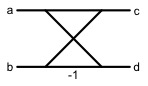
\includegraphics{gorsel/fft_radix2_butterfly.jpg} \caption{Radix 2 için butterfly işlemi}  
\end{figure}

$k_{1} = cos(-\frac{2pi}{N}) \& k_{2} = sin(-\frac{2pi}{N})$
\begin{equation} \label{equation:fft_radix2_butterfly}
  \begin{bmatrix}
    c_{Re} & c_{Im} \\[0.3em]
    d_{Re} & d_{Im} 
  \end{bmatrix} 
  = 
  \begin{bmatrix}
    a_{Re} & a_{Im} \\[0.3em]
    a_{Re} & a_{Im} 
  \end{bmatrix}
  +
  \begin{bmatrix}
    b_{Re} & b_{Re} \\[0.3em]
    -b_{Re} & -b_{Re} 
  \end{bmatrix}
  \begin{bmatrix}
    k_{1} \\[0.3em]
    k_{2} 
  \end{bmatrix}
  +
  \begin{bmatrix}
    -b_{Im} & b_{Im} \\[0.3em]
    b_{Im} & -b_{Im} 
  \end{bmatrix}
  \begin{bmatrix}
    k_{2} \\[0.3em]
    k_{1} 
  \end{bmatrix}
\end{equation} 

\begin{figure}[h] \label{image:fft_radix2_8p}
\centering 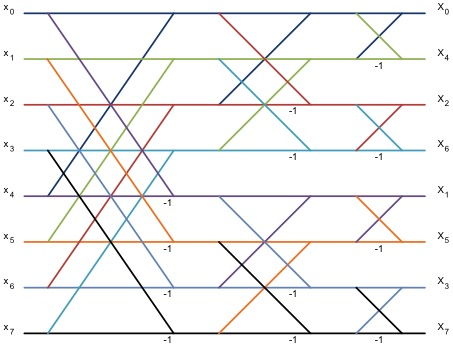
\includegraphics{gorsel/fft_radix2_8p.jpg} \caption{8 noktalı sinyal için FFT Radix 2 algoritması}  
\end{figure}

Denklem \ref{equation:fft_radix2_butterfly}'de görüldüğü üzere her bir butterfly işlemi matris çarpımları ve matris toplamları şeklinde ifade edilebilir. İşleme alınan parametreler a ve b sayılarının reel ve imajiner kısımlarının yanı sıra $sin(-2\pi/N)$ ve $cos(-2\pi/N)$ değerleridir. Burada N değeri sonuç vektörünün her bir elemanın indisi olup, bir eleman için bir kez hesaplanır. \par
FFT gerçeklemesi için sin ve cos değerlerinin hesaplanabilmesi gerekmektedir. Dolayısıyla matris çarpma ve toplama işlemlerinin yanı sıra trigonometri buyrukları da gerekmektedir.

\subsection{Logaritma}
Verilen bir veri setinin her elemanı için doğal logaritma (e tabanında) ve 10 tabanında logaritma hesaplanması gerekir. Xilinx tarafından sağlanan IPCore ile doğal logaritma hızlı bir şekilde hesaplanabilmektedir. 
$log_{a}(x) = log_{e}(x) / log_{e}(a)$ 
denkliğinden faydalanılarak herhangi tabanda logaritma hesaplanabilir. Burada buyruk kümesine $log_{e}x$ buyruğunun da eklenmesi gerekir.

\subsection{Eksponansiyel}
Verilen bir veri setinin her elemanı için $10^{x}$ ve $e^{x}$ değerlerinin hesaplanması gerekir. Xilinx tarafından sağlanan IPCore ile $e^{x}$ hızlı bir şekilde hesaplanabilmektedir. $a^{b} = e^{b x log_{e}{a]}}$ denkliğinden faydalanılarak herhangi $a^{x}$ değeri hesaplanabilir.

\subsection{Norm}
Sinyal işlemede yaygınlıkla kullanılan matris normları 1, 2 ve $\infty$ normlardır. 1-norm sütun toplamlarının maksimumu şeklinde tanımlıdır. 
$\|X\|_{1} = max_{j}(\sum_{i}(a_{ij}))$ 2-norm matrisin karesinin en büyük özdeğerinin karekökü olarak tanımlanmıştır. $\|X\|_{2} = \sqrt[2]{max(eig(AxA))}$. Bir matrisin $\infty$ normu ise satır toplamlarının maksimumu olarak tanımlanmıştır. $\|X\|_{\infty} = max_{i}(\sum_{j}(a_{ij}))$.\cite{smith1997matlab}\par
2-norm için kullanılacak özdeğerlerin hesaplanması bu işlemin bir alt parçasıdır. Özdeğer hesaplama algoritmasının gerçeklenmesinde matris büyüklüğü sabit kabul edilemeyeceği ve toplama ve kaydırma gibi temel işlemler cinsinden paralelleştirilebilir bir program yazılabileceği için özdeğer hesaplama işini yazılım seviyesinde gerçeklemek daha uygundur.\cite{eigenvalueComputation} \par

\subsection{Evrişim}
Evrişim (ing. convolution) sinyal işlemede sıklıkla kullanılan bir işlemdir. İki vektörün evrişimi $Conv(f,g)[n]=\sum_{m=-\infty}^{\infty}(f[n]xg[n-m])$ şeklinde hesaplanır. Formülden de anlaşılacağı üzere evrişim sonuç vektörünün her bir elemanı bir dizi çarpımın toplamı şeklinde hesaplanır. Burada sonuç vektörünün her bir elemanı için ayrı thread koşturulursa, 1 çarp ve N-1 çarp-topla buyruğu ile sonuç hesaplanmış olur. 

\subsection{Alt Matris, Flip, Reverse, Eşlenik ve Transpoz}
Karmaşık sayılar düzleminde a + ib şeklinde tanımlanan bir karmaşık sayının eşleniği a - ib sayısıdır. Sayısal sistemlerde karmaşık bir sayının reel ve imajiner kısımları ayrı değerler olarak tutulduğundan imajiner kısmın işaretinin değiştirilmesi eşlenik hesaplaması için yeterlidir. Transpoz işlemi ise matris elemanlarının yerlerinin değiştirilmesi yani okunup işlem yapılmadan yazılması ile gerçeklenir. Alt matris, flip ve reverse işlemleri ise yalnızca okuma ve yazma bellek işlemlerinden oluşur. 

\subsection{Determinant}
Genel geçer determinant hesaplama yönteminde matris, 2x2 boyutunda alt parçalarına ayrılır determinantlarından yeni bir matris oluşturulur, oluşan matris üzerinde yine aynı işlem uygulanır. En son tek elemana düştüğünde matrisin determinantı hesaplanmış olur. 2x2 matrisin determinantı $det(A) = a_{00} x a_{11} + a_{01} x a_{10}$ şeklinde hesaplanır. Bu işlem 1 çarpma 1 çarp-topla buyruğu ile gerçeklenebilir.

\subsection{Trigonometrik İşlemler}
Tüm trigonometrik işlemler sin ve cos cinsinden ifade edilebilir. FPGA platformunda Xilinx IPCore kullanılarak sin ve cos işlemleri hızlıca hesaplanabilir. 

\subsection{Filtreleme ve Windowing}
Filtreleme ve windowing işleminde önceden belirlenmiş bir vektör veya matris işleme alınacak vektör yada matris üzerinde gezdirilerek eleman eleman çarpma ve toplama işlemleri yapılır. Gereksinimlerde belirtilen Hamming Hanning Gaussian windowing işlemlerinde window değişir, işlem aynıdır. FIR ve IIR filtrede de temel işlemler windowing ile aynı olup, algoritma seviyesinde farklılıklar ile gerçeklenir. Bir f vektörü üzerine uygulanacak g maskesi ile filtreleme veya windowing $y[n] = \sum_{i=0}^{N}f[i]xg[i]$ şeklinde gösterilebilir. 

\subsection{Türev}
Bir vektörün türevi, ayrık zamanda ardışık elemanların farkı şeklinde tanımlıdır. N elemanlı bir vektörün türevinin hesaplanması için N adet thread oluşturulur ve her bir thread bir çıkarma işlemi yapar. 

\subsection{Sıralama}
Satır, sütun ve matris elemanlarının sıralanması uygulaması herhangi bir sıralama algoritması ile gerçeklenebilir. Alt seviyede her bir thread  basit karşılaştırma işlemleri yapar.

\subsection{Varyans ve Standart Sapma}
Varyans ve standart sapma için dizinin ortalaması hesaplanır, elemanların ortalamaya uzaklıkları üzerinden toplama, karesini alma ve karekök alma gibi işlemler yapılır. 

\subsection{Karekök}
Karekök işlemi kendi başına bir uygulama olarak değil diğer uygulamaların içinde bir işlem olarak kendini gösterir. Xilinx IPCore kullanılarak karekök işlemi hızlı bir şekilde yapılabildiğinden IPCore kullanımı tercih edilmiştir.

\subsection{İşaret}
İşaret fonksiyonu bir matris veya vektörün tüm elemanları için eleman pozitif ise 1, 0 ise 0, negatif ise -1 değerini döndürür. Eleman sayısı adetinde thread oluşturularak hızlı bir şekilde bu işlem gerçekleştirilebilir.

\subsection{Interpolasyon}
Interpolasyon işlemi, ardışık elemanların ağırlıklı ortalamalalarının hesaplanması ile gerçeklenir. Temel toplama, çarpma, kaydırma, bölme gibi işlemler ile ağırlıklı ortalama hesaplanır. Eleman sayısı kadar thread oluşturularak işlem paralelleştirilebilir.

\subsection{Özet}
Listedeki fonksiyonların incelenmesi ile gerekli hesaplama buyrukları çıkarılmıştır. Fonksiyon listesinin gerçeklenebilmesi için gerekli buyruklar Tablo \ref{table:instructionList1}'de sunulmuştur. 

\begin{longtable}{p{80pt} p{250pt}}
\caption[Desteklenmesi beklenen fonksiyon listesi]{Desteklenmesi beklenen fonksiyon listesi} \label{table:fonksiyonListesi} \\
\multicolumn{1}{c}{\textbf{Fonksiyon}} & \multicolumn{1}{c}{\textbf{Açıklama}} \\ 
\hline 
\endfirsthead

\multicolumn{2}{c}%
{{\bfseries \tablename\ \thetable{} -- devam}} \\
\multicolumn{1}{c}{\textbf{Buyruk}} &
\multicolumn{1}{c}{\textbf{Detay}}  \\ \hline 
\endhead

\hline \multicolumn{2}{r}{{Sonraki sayfada devam etmektedir.}} \\ 
\endfoot

\hline \hline
\endlastfoot
  and, or, not,    &    \\

 Karşılaştırma          & Satır, sütun bazlı veya matris için karşılaştırma           \\%math_desc    & 
\end{longtable}